\graphicspath{{./lab00/Images/}}

\maketitlepage{App Development}{in Android Studio}{Lab 0: First Project}
\maketocpage

\section{Android}
\subsection{What is Android?}
Android is a partially open source\footnote{It is shipped with some proprietary software, \href{https://play.google.com/store?hl=en}{Google Play Store} for example} Linux based software stack maintained by Google. It runs on a wide variety of devices, including mobile phones, tablets, TVs, watches and cars. The software stack's layers as well as some of their components can be seen in figure \ref{fig:droidarc}.

\begin{figure}[H]
\centering
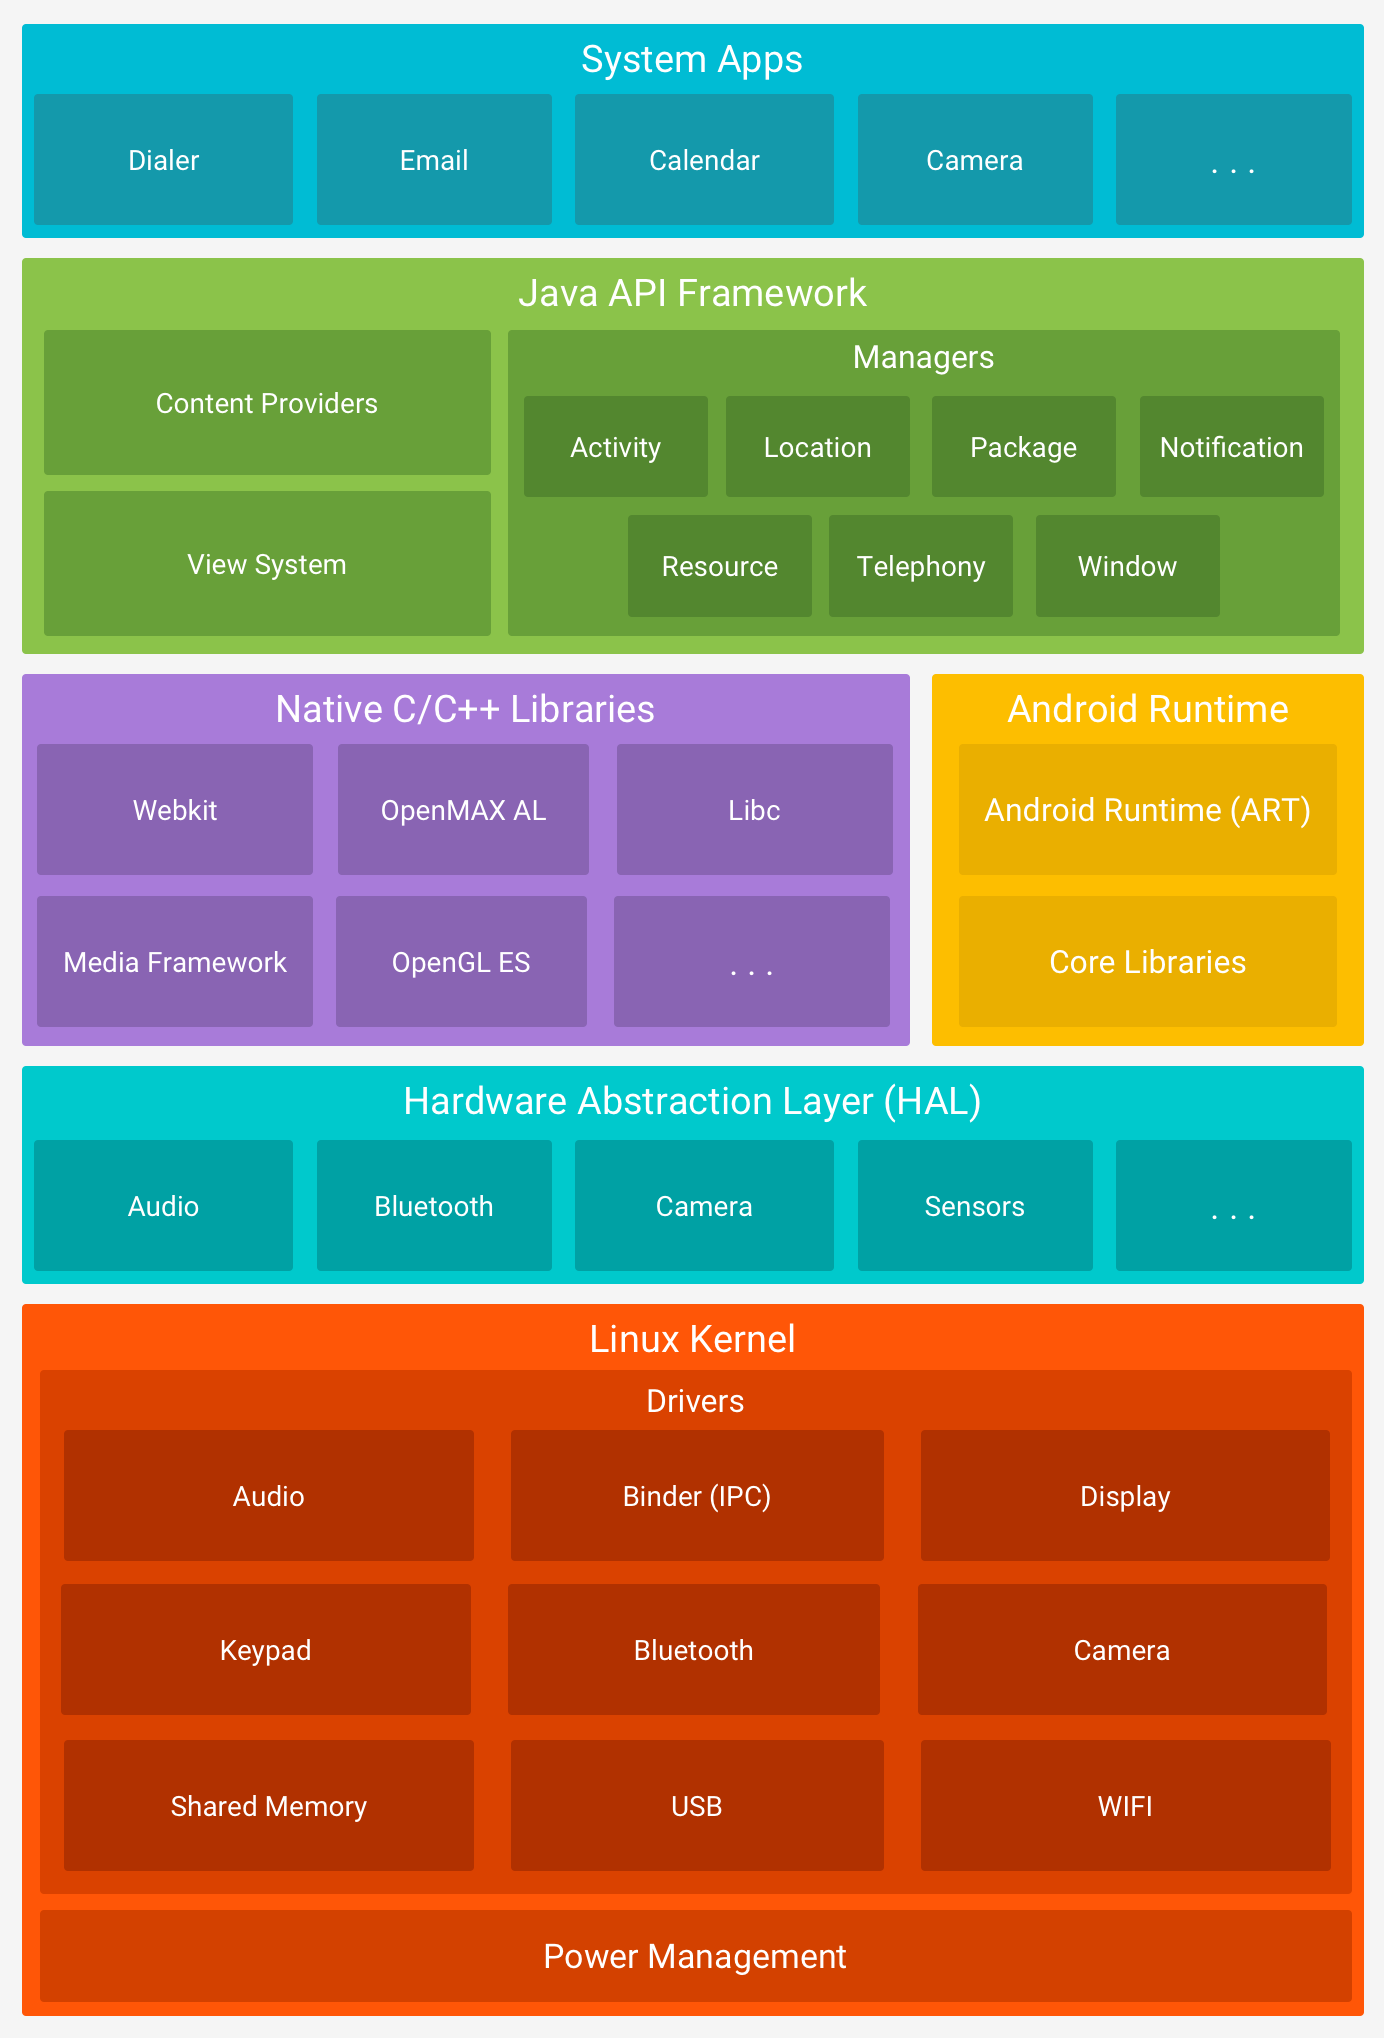
\includegraphics[scale=.3]{android_architecture_detailed.png}
\caption{The Android platform}
\label{fig:droidarc}
\end{figure}

\fat{The Linux Kernel} 
At the bottom of the stack is the Linux kernel. Neither users or app developers interact with this layer directly. This layer contains drivers for various device hardware and allows their manufacturers to develop them for a known kernel. This layer also handles low level memory management, networking, power management, process management, threading, file system management and security, for example.\\

\fat{Hardware Abstraction Layer (HAL)} 
The HAL defines a standard interfaces for inconsistent hardware vendors to implement. Any hardware intending on using Android must implement drivers and HAL interfaces for each hardware component. This provides a standardized link from upper levels of the stack down to the drivers. There is no specification on how HAL and drivers interact which is left to the vendors. HAL implementations are packaged into modules and loaded by the Android system at the appropriate time.\\

\fat{Android Runtime}
Compilation and execution of Java code happens in this layer. The virtual machine that Java typically uses (JVM) is not used by Android which uses its own instead. Prior to Android 4.4 it used a virtual machine called Dalvik\footnote{Named after a town in Eyjafjörður, Iceland} which used a just-in-time compilation (JIT). Android 4.4 brought with it Dalvik's replacement, Android RunTime (ART) which added ahead-of-time (AOT)\footnote{It began by replacing it but JIT was later reintroduced} compilation and improved garbage collection. The \href{https://developer.android.com/reference/classes.html}{core libraries} contains a subset of Java's standard library (e.g. \texttt{java.util} and \texttt{java.lang}) as well as some Android specific core Java libraries (e.g. \texttt{android.app}, \texttt{android.database}, \texttt{android.opengl} and \texttt{android.util}).\\

\fat{Native \texttt{C}/\texttt{C++} Libraries}
Both the hardware abstraction and Android runtime layers are implemented in \texttt{C}/\texttt{C++} (while the kernel is written in \texttt{C} and assembly language). Most of the Java and Android core libraries have corresponding functionality implemented in \texttt{C}/\texttt{C++} and available to the other Java layers through the Java Native Interface (JNI). Among the libraries included are OpenGL ES for graphics, SSL for secure networking and the system library libc.\\

\fat{Java API Framework}
The Application Framework is the collection of services where Android applications are run and managed. Some of the services provided are the Activity Manager which manages application lifecycle and the activity stack and Content providers that provide apps with a way to access data from other apps.\\

\fat{System Apps}
The final layer contains the applications that come with the Android platform. These include apps like SMS messenger, Contacts, Camera and Phone. These apps are both useful for standalone usage as well as supporting other applications.

\subsection{A very brief history of Android}

\begin{minipage}{0.33\textwidth}
Android Inc. was founded in 2003 by Andy Rubin, Rich Miner, Nick Sears, and Chris White. Its original purpose was to create an operating system for digital cameras but soon shifted its goal towards the mobile phone market. In 2005 Android Inc. was acquired by Google along with its key employees. Three years later the first mobile phone using Android was released, the T-Mobile G1 or HTC Dream, seen in figure \ref{fig:htc}.
\end{minipage}
\hfill
\begin{minipage}{0.60\textwidth}
\begin{figure}[H]
\centering
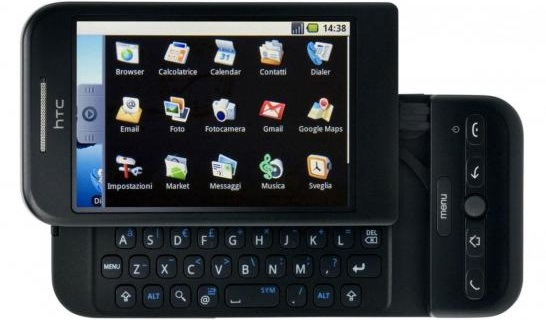
\includegraphics[scale=.75]{htc_dream.jpg}
\caption{T-Mobile G1}
\label{fig:htc}
\end{figure}
\end{minipage}
\\

Since then, a new version of Android has been released regularly, that consistently add to its feature list. What version support which feature is something we must pay attention to.

\begin{table}[H]
\centering
\begin{tabular}{c|l|c|l}
Version number & Initial release date & API level & Code name \\
\hline
$1.0$ & September, 2008 & 1 & \\
$1.1$ & February, 2009 & 2 & \\
$1.5$ & April, 2009 & 3 & Cupcake \\
$1.6$ & September, 2009 & 4 & Donut \\
$2.0$-$2.1$ & October, 2009 & 5-7 & Eclair \\
$2.2$-$2.2.3$ & May, 2010 & 8 & Froyo \\
$2.3$-$2.3.7$ & December, 2010 & 9-10 & Gingerbread \\
$3.0$-$3.2.6$ & February, 2011 & 11-13 & Honeycomb \\
$4.0$-$4.0.4$ & October, 2011 & 14-15 & Ice Cream Sandwich \\
$4.1$-$4.3.1$ & July, 2012 & 16-18 & Jelly Bean \\
$4.4$-$4.4.4$ & October, 2013 & 19-20 & KitKat \\
$5.0$-$5.1.1$ & November, 2014 & 21-22 & Lollipop \\
$6.0$-$6.0.1$ & October, 2015 & 23 & Marshmallow \\
$7.0$-$7.1.2$ & August, 2016 & 24-25 & Nougat \\
$8.0$ & August 2017 & 26 & Oreo 1\\
\end{tabular}
\caption{Android version history}
\label{table:droidvers}
\end{table}

\subsection{Why Android?}
There are other platforms to consider, like iOS and Microsoft. Most of the largest mobile apps are available for all major platforms but if you could only choose one, Android's market share provides a convincing argument. It is by far the largest in the mobile market and that also holds for the most traffic when it comes to app downloads. If you are looking to get your project noticed, these are facts to consider.\\

There are also web applications which smart phones can run with their web browser. Studies show that a vast majority prefers apps over web applications when using mobile phones and tablets. Apps have better access to the phone resources and tend to have a nicer UI. One could argue that web applications are therefore serving a different market.\\

There are no right or wrong answers here so one must come to his or her own conclusion whether to prefer Android over something else. Each project is unique and for some Android might be perfect while not so much for others. 

\section{Android Development}
The biggest decision when it comes to Android development is whether to develop native Android apps or cross platform. Both approaches bring pros and cons. Developing native Android apps has only one flaw but it might be considered a big one. The app will not run on any other devices. Developing natively will give direct API access, better performance and development with Java and Android Studio.\\

React native and Xamarin are among the cross platform approaches, using javascript and \texttt{C\#} respectively. Another approach is to host your app's logic on a web server and create native UI for whatever platform you want to support. Again, there are no general best choices. You must evaluate what approach is best for the task at hand as well as your skills and preferences. That being said, the native approach will be our choice in this course.\\

To develop Android apps natively we need The Android software development kit (SDK) and some device to run our app on. We will also use Android Studio as an IDE in this course although that is not required to write apps (but highly recommended). It is Google's official Android IDE\footnote{which had been Eclipse priror to Android Studio release in 2014}, based on IntelliJ.

\section{Setup}
Download Android Studio (available \href{https://developer.android.com/studio/index.html}{here}) and follow the installation instruction (\href{https://developer.android.com/studio/install.html}{here}) for your operating system.

\section{Create a project}
\begin{itemize}
\item Create a new project. You do not need \verb!C++! support.
\item Select minimum SDK of at least 21. Only select the phone and tablet module.
\item Select an empty activity. Make sure to auto generate layout and choose \verb!AppCompat!.
\end{itemize}

\section{Structure of the project}
The project structure for a new project with an empty activity can be seen in figure \ref{fig:prstr}.

\begin{figure}[H]
\centering
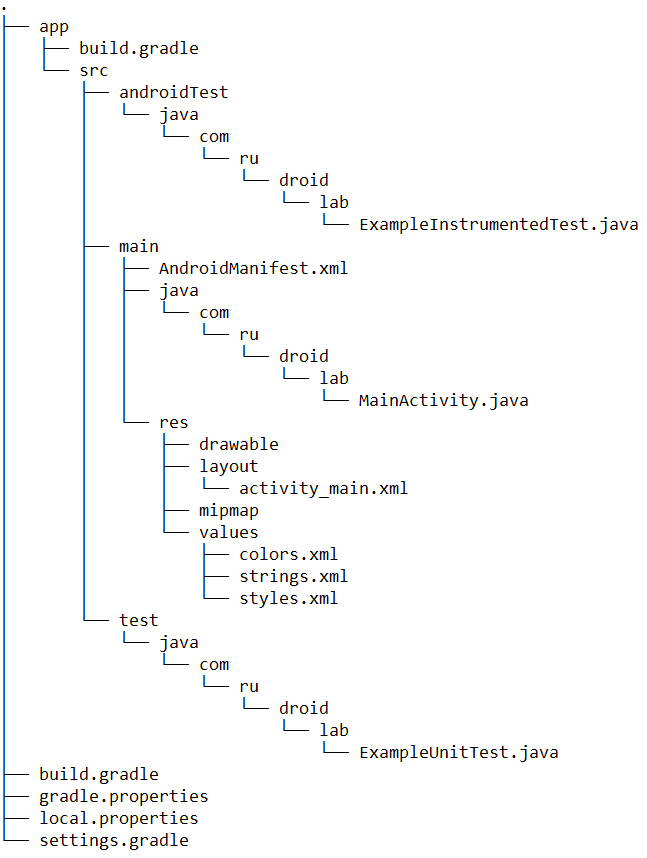
\includegraphics[scale=.75]{project_structure.png}
\caption{Project structure}
\label{fig:prstr}
\end{figure}

\begin{itemize}
\item \textbf{Gradle} is your build configuration.
\item \textbf{Manifest} contains the file \verb!AndroidManifest.xml! which every project requires. It contains various information required to run the app such as components and permissions.
\item \textbf{src/test} contains unit test that do not need Android to run.
\item \textbf{src/androidTest} contains instrumented test that do require Android to run.
\item \textbf{src/main/java} contains the source code of your app.
\item \textbf{src/main/res} contains your resource files, including UI strings, layouts and drawable files. 
  \begin{itemize}
      \item \textbf{drawable} contains images.
      \item \textbf{layout} describes UI layout.
      \item \textbf{mipmap} contains drawable icons.
      \item \textbf{values} holds constant values.
  \end{itemize}
\end{itemize}

\section{The first app}
Start by finding \verb!strings.xml! in \menu{app > res > values} and add the following string.
\begin{lstlisting}[style=A_XML]
<string name="hello">Hello World!</string>
\end{lstlisting}
Every UI string should always be stored in this file. Doing that makes it easier to update their values as well as being Android's way to localize. Find the generated layout for the empty activity you created in \menu{app > res > layout} and add the following code.
\begin{lstlisting}[style=A_XML, caption={Hello World view}, label = {listing:hwv}]
<TextView
    android:layout_width="wrap_content"
    android:layout_height="wrap_content"
    android:text="@string/hello"
    app:layout_constraintBottom_toBottomOf="parent"
    app:layout_constraintLeft_toLeftOf="parent"
    app:layout_constraintRight_toRightOf="parent"
    app:layout_constraintTop_toTopOf="parent" />
\end{lstlisting}

\section{Run}
You can choose any method you want to run the app but in general, it is a good idea to try it on more than one device. We do require all labs to work for multiple phones.

\subsection{Built in Emulators}
To create a new device, click on the AVD manager shown in figure \ref{fig:avd} and then 'Create Virtual Device'. Pick what device and Android version you want and proceed. If not enabled already, you might have to enabled the Virtualization(VT) in BIOS.
\begin{figure}[H]
\centering

\includegraphics[scale=1]{AVD_MAN.png}
\caption{AVD manager}
\label{fig:avd}
\end{figure}

\subsection{Using an Android phone}
In order to run our program on an actual Android device we need enable USB Debugging in Developer options. It is hidden by default and it depends on your operating system how to display it. On Android 4.2 and higher, it can be done by tabbing the build number 7 times, found in \menu{Settings > About phone}.

\subsection{Third party emulators}
The most popular third party emulator for Android development is \href{https://www.genymotion.com/}{Genymotion} but it is not free. There are many alternatives out there which you can explore although most are probably not tailored for development. You do need to watch out for any limitation before choosing one as some might not support all features we will use.
